\documentclass[sigconf,anonymous,review,balance=false]{acmart}
\usepackage{booktabs}
\usepackage{listings}
% Allow a final line-breaking pass for narrow columns; no margin/font changes.
\setlength{\emergencystretch}{1em}
\lstset{basicstyle=\ttfamily\footnotesize,breaklines=true,columns=fullflexible,keepspaces=true,showstringspaces=false,frame=single,captionpos=b}
\setcopyright{none}
\acmConference[WWW '27]{The ACM Web Conference 2027}{May 10--14, 2027}{Dublin, Ireland}
\acmYear{2027}
\acmDOI{}
\acmISBN{}
\title[Structural Selection Profiles and Relational Evidence]{From Tool Selection to Knowledge-Graph Entity Selection: Structural Profiles and Relational Evidence}
\begin{document}
\begin{abstract}
Tool-selection success varies with the pattern of dependencies between tools, motivating questions about which structural difficulties persist when relations are explicitly supplied. We revisit this problem through archived knowledge-graph entity selection on seven task families and three language models. Building on a prior Tool-to-KG study, we distinguish adding relational evidence from changing the presentation of matched facts and introducing adjacent distractors. Recall is the primary metric for recovery of the entity-route reference, with precision and exact recovery providing complementary diagnostics. Adding relations increases mean recall by 0.774, 0.519, and 0.567 for Gemma, Qwen, and Ministral. Residual profiles depend on task family, size, and model. On six-node incoming trees, Qwen recall is 0.603 with source-card relations and 0.802 when the same facts appear on both endpoint cards; moving them to destination cards alone leaves recall at 0.603. Output-level analyses retain both corrections and regressions under presentation changes. The findings distinguish relation availability from complete route recovery and refine hypotheses about structural selection errors without asserting a universal topology ranking or shared causal mechanism.
\end{abstract}
\ccsdesc[500]{Information systems~Information retrieval}
\ccsdesc[300]{Computing methodologies~Natural language processing}
\keywords{knowledge graphs, tool selection, entity selection, relational evidence, graph patterns}
\maketitle
\section{Introduction}
\label{sec:intro}
Selecting the right elements from a catalogue is a prerequisite for many language-model agents that access Web information. A tool-using agent must retain the operations needed to satisfy a request; a knowledge-grounded system must retain the entities that connect a question to its supporting facts. In either setting, choosing individually plausible names can omit intermediate context, while selecting too broadly can introduce irrelevant elements. Understanding selection reliability therefore requires examining how the requested elements compose.

Tool Graph Complexity reports that tool-selection success differs across dependency patterns, beyond what the number of reference tools alone describes~\cite{anonymousToolGraph}. Its controlled analysis retains a sequential-pattern penalty after accounting for measured size and surface properties. This motivates a question about the source of structural difficulty: does a pattern remain difficult when its relations are explicitly supplied, or does part of the difficulty arise from recovering dependencies from descriptions?

The same work investigates this question using a knowledge graph (KG) in Appendix~O. It reports partial structural transfer, an easier explicit-KG Chain profile, residual incoming-tree difficulty, and adjacent-decoy errors~\cite{anonymousToolGraph}. These antecedent observations motivate examining which errors remain after relation disclosure and how evidence conditions constrain their interpretation.

We address this question through an archived corporate-KG entity-selection study. The graph connects companies, people, products, locations, and news and was developed for corporate GraphRAG evaluation~\cite{kirpichev2026towards}. Our Web-related concern is the reliability of selecting connected evidence for querying interlinked corporate information: a route can be incomplete even when plausible endpoint entities are retained. We evaluate recovery of a declared entity-route reference, separating this access step from final answer correctness.

Our analysis distinguishes three comparisons. Raw versus Raw+E adds explicit relations to otherwise matched entity cards. Controlled triples versus templated prose and alternative card hosting retain designated facts while changing their presentation. Adjacent-context pairs add connected but query-irrelevant distractors. Keeping these contrasts separate matters: an information gain cannot be interpreted as merely an encoding effect, and complete route coverage is not the same objective as finding one sufficient answer.

We ask: \textbf{RQ1}, how do entity-selection profiles vary with task family and reference size? \textbf{RQ2}, how do relation availability, fact presentation, and adjacent contexts change recall and residual errors? \textbf{RQ3}, what do these observations imply for the interpretation of Tool-to-KG structural transfer? RQ3 is a descriptive comparison with prior evidence, not a new matched cross-domain experiment.

The additional contribution is a diagnostic follow-up: (i) separating relation disclosure from fact-preserving presentation, and (ii) localizing residual omissions, excess selection, and same-task presentation sensitivity. Family and size profiles provide its structural context. Recall is primary; precision and exact distinguish selectivity and complete-set recovery. This is an empirical analysis of an existing KG, without a new algorithm or resource claim. Exact task/response overlap with Appendix~O is unquantified; we do not claim independent replication.

The results show why relation visibility is insufficient as a complete explanation. Disclosure substantially increases recall, yet residual profiles differ across families and models. On six-node incoming trees, Qwen retains high precision but incomplete recall; repeating the same relations across both endpoint cards increases recall more than moving them to destination cards alone. Contrary model outcomes and regressions remain visible. These observations constrain possible explanations of selection errors without identifying a shared internal mechanism for tools and KG entities.

\section{Related Work and Prior Transfer Evidence}
\label{sec:related}
\paragraph{Structural difficulty in tool selection.}
Tool Graph Complexity separates reference-set minimality from dependency composition and reports motif-associated differences in selection success~\cite{anonymousToolGraph}. Its size-adjusted sequential penalties should not be conflated with every motif's raw difficulty: the adjusted Tree-in interval includes zero relative to Star-out. Appendix~O already evaluates KG motifs, size, explicit relations, and adjacent decoys. Its Chain inversion and residual incoming-tree interpretation are antecedent findings, not discoveries claimed here. Our increment concerns archived relation-availability and matched-fact presentation contrasts and more localized output-level diagnostics. Different references, prompts, populations, and model protocols prevent direct cross-paper score subtraction.

\paragraph{Graph representation and task comprehension.}
Talk like a Graph establishes that graph encodings, task type, and structure affect LLM performance~\cite{fatemi2024talklikegraph}. Dai et al. investigate terminology- and topology-based pattern comprehension and discovery~\cite{dai2025graphpatterns}. Our output is a set of entities covering all permitted query routes, rather than a motif label or one discovered pattern. This task distinction does not make representation sensitivity itself novel.

\paragraph{KG evidence and traversal failures.}
KG-prompt research studies input formats, triple organization, and noisy or incomplete evidence, including answer-based evaluation~\cite{dai2024kgunderstanding}. GraphWalk studies tool-mediated navigation and reports incomplete exploration in graph-context settings~\cite{ghandi2026graphwalk}. Accordingly, we do not claim the first observation of incomplete traversal. We measure final-set signatures and changes on the same archived tasks; these are not execution traces. The corporate graph and earlier QA benchmark belong to Kirpichev et al.~\cite{kirpichev2026towards}; graph construction and downstream QA gains are outside our contribution.

\section{Task, Reference, and Relational Evidence}
\label{sec:method}
\paragraph{Source graph and historical scope.}
We reuse the corporate KG snapshot described by Kirpichev et al.~\cite{kirpichev2026towards}, covering S\&P~500 companies and associated sectors, industries, executives, investors, products, resources, locations, and news. The authors confirm unchanged snapshot reuse. We analyze the archived, frozen tasks rather than reconstruct their historical database extraction from current software. Appendix~\ref{app:cypher} reproduces the author-supplied Cypher extraction specification. It defines fixed small instances and an induced-edge filter; it is not presented as the complete executable pipeline for all archived sizes or per-cell sampling quotas. No database query was executed during this analysis.

\subsection{Directed Task Families}
\label{sec:motifs}
We study seven directed families: chain, star-in, star-out, tree-in, tree-out, rhombus, and hourglass. Figure~\ref{fig:raw_motifs} gives a compact key alongside Raw/Raw+E recall. Arrows denote factual KG relations; incoming queries inspect them in the reverse direction. Each query names an anchor, which belongs to the all-route selection reference together with the endpoints and intermediate entities. Stars use one-link incoming or outgoing queries; trees and rhombi use two-link routes, ending earlier only at a dead end. Chains stop at the first requested entity type, and hourglass queries request incoming and outgoing one-link groups separately. The Core sizes are six nodes for chain, stars, and trees, four for rhombus, and five for hourglass. Full graph definitions, traversal rules, and the distinction between endpoint answers and selected route entities appear in Appendix~\ref{app:motifs}. The families also differ in query operations and entity/relation types.


\paragraph{Candidates and distractors.}
Each main task presents 25 named candidate entities, including the motif entities and distractors. Disconnected distractors have no edges to reference entities in either direction, although they may connect to each other. In the adjacent variant, up to ten distractors are neighbours of motif entities; remaining distractors are disconnected. Paired noise variants retain the question and reference but may contain different distractor identities. Explicit evidence includes relations involving distractors, not only reference-induced edges.

\paragraph{Selection target.}
Let $C$ denote the candidate catalogue and $G_C$ its graph-defined reference context, which need not be recoverable from native cards. Let $q$ be the endpoint query, $a$ its anchor, and $\mathcal{P}(q,G_C)$ its allowed supporting routes under the saved traversal/stopping rule. We evaluate the entity-route reference
\begin{equation}
 W(q,G_C)=\{a\}\ \cup\!\bigcup_{p\in\mathcal{P}(q,G_C)} V(p),
\end{equation}
where $V(p)$ contains every entity on route $p$. Endpoint answers $A(q,G_C)$ are distinct from $W$. Simple routes do not revisit an entity; the saved task specification fixes the allowed direction, depth, and terminal-type rule. In the audited structured archive, saved motif/reference IDs coincide with this witness union. Equality is a property of these accepted tasks, not an assumed identity for arbitrary candidate expansion.

For example, one archived rhombus has two branches from the anchor through two intermediate entities to one endpoint. Its endpoint answer has one entity and its reference four. Removing the endpoint card's facts while retaining the name/type catalogue leaves that endpoint recoverable from incoming facts. Thus reference membership does not establish that every card contributes indispensable information. The selection objective is complete route coverage, not minimum sufficient evidence or final answer correctness.

\paragraph{Evidence conditions.}
Raw presents original entity metadata; Raw+E adds explicit relations to the same cards. Actual archived inputs, questions, candidate order, and references match after removing only the relation fields. This is an information-availability contrast; native descriptions are not assumed to express all graph relations. Controlled triples and templated prose instead encode designated matched graph facts. Source-card, destination-card, and both-card variants alter presentation location while retaining relation direction. Names/types remain visible in all conditions. Pseudonyms, direct questions, and linked-attribute encodings provide further diagnostic contrasts detailed in Appendix~\ref{app:conditions}.

\section{Experimental Design and Evaluation}
\label{sec:setup}
\paragraph{Archived models and populations.}
We analyze Gemma-4-31B, Qwen3.6-Flash, and Ministral-14B as identified in the archive. Core has 700 base tasks, with 100 in each of seven families, under 13 conditions. Five families have six nodes; rhombus and hourglass retain four and five. Full Raw/Raw+E has 3,400 bases per condition/model: chain sizes 3--6, stars 3--10, trees 5--10, rhombus four, and hourglass five, totaling 34 motif-size cells of 100 tasks. All main candidate pools contain 25 entities.

The 700 Core base IDs also occur in Full Raw/Raw+E. Models and conditions reuse base tasks, so counts across panels are not independent replications. Sizes are different frozen cohorts rather than paired expansions of one graph. The separate additional-size and incremental panels are supplementary and are not pooled into the main comparisons.

\paragraph{Comparisons.}
RQ1 uses Core source-card triples with disconnected (K1) and adjacent (K2) distractors and the Full size grid. RQ2 compares Raw with Raw+E, matched triples with text, and hosting on source, destination, or both cards. K1, K3, and K4 retain a procedural question; K7 uses a direct formulation of the same endpoint query with source-card triples. K5 and K6 are the text counterparts of disconnected and adjacent conditions; K8 uses text with a direct query. Core K-conditions use pseudonyms. Archived inputs establish pairing and fact invariants, independently of current builder defaults.

\paragraph{Responses and evidence coverage.}
The main protocol requests JSON with selected catalogue names and an insufficient-evidence flag. Valid selections contain exact, unique candidate names; the flag does not modify set scores. Available Qwen/Ministral records specify OpenRouter, temperature zero, a 1,024-token limit, and JSON-object formatting. Missing Gemma settings are not filled from current defaults. Some controlled Gemma outcomes retain cached individual metrics without original replies or selected identities; these support aggregate recall, precision, and exact recovery, but not identity-level route signatures. Full Raw/Raw+E has stronger reply coverage. Missing and invalid outcomes remain in planned denominators.

\paragraph{Primary and additional metrics.}
For selected set $S$ and nonempty route reference $W$, we use
\begin{equation}
 R(S,W)=\frac{|S\cap W|}{|W|},\qquad
 P(S,W)=\frac{|S\cap W|}{|S|}.
\end{equation}
An empty selection receives zero recall and precision. Recall is primary because the selection target requires complete route coverage. Precision measures excess selection; exact recovery is one only when $S=W$. We report macro means of individual scores over all planned outcomes, with invalid/missing outcomes contributing zero. Thus scores also reflect protocol reliability; they are not pooled micro ratios or valid-only summaries. Reference coverage is distinct from endpoint-answer correctness and minimal sufficient evidence.

\paragraph{Analysis and uncertainty scope.}
The figures and tables use saved aggregate scores and existing bounded selection diagnostics; this revision launches no model, judge, or database calls. Core condition contrasts match 700 bases per model; Raw/Raw+E matches 3,400. Differences are right-minus-left macro means on these complete paired populations. Source-row mappings reproduce the existing paired export. Recall/precision profiles and contrasts are descriptive: no new confidence intervals, significance claims, or motif-by-condition tests are introduced. Earlier uncertainty estimates cover F1/exact, and are not transferred to recall. Repeated anchors and shared entities further restrict population inference.

\section{Results}
\label{sec:results}
\subsection{Structural Profiles: Motif and Size}
\begin{figure*}[t]
\centering
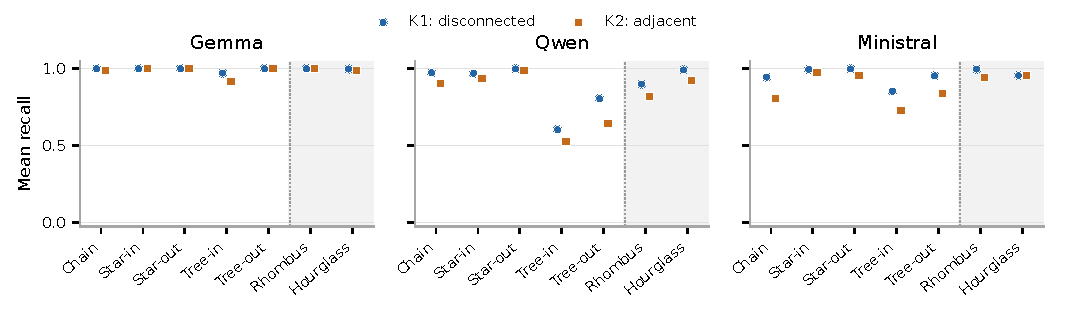
\includegraphics[width=\textwidth]{figures/recall_motifs.pdf}
\caption{Core recall with explicit source-card relations: K1 disconnected and K2 adjacent distractors, 100 planned tasks per point. The first five families have six nodes; shaded rhombus/hourglass use four/five and are not equal-size contrasts. Invalid outcomes contribute zero. These are descriptive macro means, without inferential error bars.}
\Description{Recall across seven graph-pattern families for three models. Incoming-tree recall is below outward-star recall, with model-dependent changes under adjacent contexts.}
\label{fig:motifs}
\end{figure*}
Figure~\ref{fig:motifs} shows task-family differences at a common reference size. Under K1, six-node incoming-tree recall is 0.972 for Gemma, 0.603 for Qwen, and 0.853 for Ministral. Outward stars are close to complete coverage. The common size does not eliminate differences in query semantics, relation types, or sampled entities; it rules out a node-count-only description of these observed task profiles, not every competing explanation.

Precision supplies a different view. Qwen's K1 incoming-tree precision is 0.988, despite recall of 0.603 and exact recovery of 0.150. It often selects a small, mostly reference-consistent set while failing to cover the reference. Gemma's corresponding precision is 1.000 and exact 0.870. Appendix~\ref{app:conditions} reports precision profiles separately rather than combining the two quantities into one F1 curve.

\begin{figure*}[t]
\centering
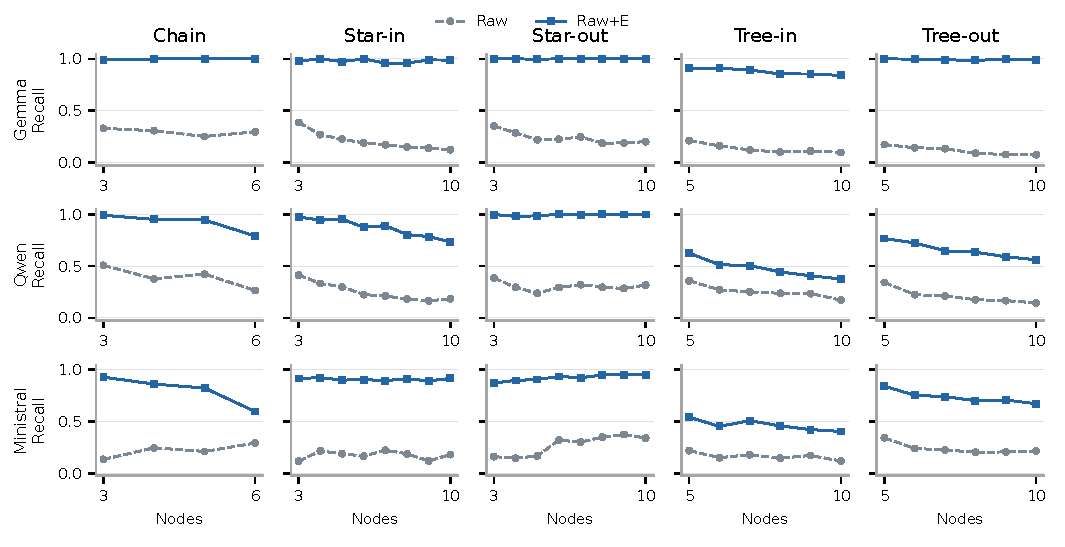
\includegraphics[width=\textwidth]{figures/recall_sizes.pdf}
\caption{Recall across all variable-size families and all three models in Full Raw/Raw+E. Each point has 100 planned tasks and 25 candidates, with invalid outcomes contributing zero. Raw+E adds relations. Sizes are different frozen cohorts, not paired expansions; target prevalence and distractor count change with size. No universal monotonicity or isolated size effect is claimed.}
\Description{Fifteen panels compare Raw and Raw+E recall against subgraph size. Incoming trees and some chains decline, while outward stars often remain near complete coverage.}
\label{fig:sizes}
\end{figure*}
Size sensitivity also depends on family and model (Figure~\ref{fig:sizes}). Under Raw+E, chain recall changes from 0.990 at three nodes to 0.790 at six for Qwen, and from 0.927 to 0.595 for Ministral. Gemma changes from 0.990 to 1.000. Outward stars provide contrary profiles: Qwen changes from 0.997 at three nodes to 0.998 at ten, Gemma remains at 1.000, and Ministral changes from 0.870 to 0.950. These comparisons describe different accepted cohorts, not beneficial or harmful effects of adding a node to the same task.

Incoming-tree Raw+E recall is lower at ten than five nodes for all three models: 0.910 to 0.841, 0.624 to 0.375, and 0.540 to 0.403 for Gemma, Qwen, and Ministral. Intermediate values need not be monotonic. The fixed candidate pool also changes the proportion of reference entities as size increases. We therefore report the full profiles, including exceptions, rather than treating node count as an intrinsic complexity coefficient.

\subsection{Relation Availability and Matched-Fact Presentation}
\begin{table*}[t]
\caption{Descriptive paired changes in mean recall. Columns: Raw+E minus Raw (3,400 pairs/model); adjacent minus disconnected triples/text; text minus triples for procedural/direct queries; destination minus source; both cards minus source; direct minus procedural query (700 pairs/model for these Core contrasts). All planned outcomes are retained. No recall confidence intervals or significance tests were computed.}
\label{tab:effects}
\centering\small
\begin{tabular}{lrrrrrrrr}
\toprule
Model & \shortstack{Raw+E} & \shortstack{Adj.\\triples} & \shortstack{Adj.\\text} & \shortstack{Text\\steps} & \shortstack{Text\\direct} & \shortstack{Dest.} & \shortstack{Both} & \shortstack{Direct\\query} \\
\midrule
Gemma & +0.774 & -0.011 & -0.015 & -0.002 & -0.006 & +0.000 & -0.003 & +0.001 \\
Qwen & +0.519 & -0.071 & -0.064 & -0.035 & -0.035 & +0.005 & +0.059 & -0.003 \\
Ministral & +0.567 & -0.072 & -0.045 & -0.001 & -0.002 & -0.043 & -0.006 & -0.016 \\
\bottomrule
\end{tabular}

\end{table*}
Explicit relation disclosure substantially increases recall (Table~\ref{tab:effects}). Raw/Raw+E mean recall changes from 0.198 to 0.972 for Gemma, 0.278 to 0.798 for Qwen, and 0.218 to 0.785 for Ministral. The gains are 0.774, 0.519, and 0.567. Precision changes from 0.859 to 0.988, 0.885 to 0.975, and 0.459 to 0.976, respectively. High Raw precision can therefore coexist with low route coverage. Since native metadata is not verified sufficient for every route, low Raw recall is not automatically a failure to reason from available facts.

Matched-fact representation gives a more restricted diagnostic. Text-minus-triples recall differences for Qwen are $-0.035$ under both procedural and direct queries after rounding. Gemma and Ministral have smaller descriptive differences in those comparisons. Hosting effects are model-specific: duplicating facts yields a Qwen aggregate recall gain of 0.059, whereas Gemma and Ministral do not show the same positive direction. These are point estimates, not equivalence findings or newly tested interactions.

\begin{table}[t]
\caption{Mean recall on six-node Tree-in tasks: one model per row, conditions in columns. K1/K3/K4 host triples on source/destination/both cards with a procedural query; K7 uses source cards and a direct query. Each cell retains 100 planned tasks. Ministral has 99 valid outcomes in K3 and 91 in K7; every other cell has 100. Invalid outcomes contribute zero.}
\label{tab:treein}
\centering\small
\begin{tabular}{lrrrr}
\toprule
Model & K1 & K3 & K4 & K7 \\
\midrule
Gemma & 0.972 & 0.983 & 0.982 & 0.982 \\
Qwen & 0.603 & 0.603 & 0.802 & 0.660 \\
Ministral & 0.853 & 0.787 & 0.908 & 0.837 \\
\bottomrule
\end{tabular}

\end{table}
The focused incoming-tree comparison illustrates why aggregate changes need localization (Table~\ref{tab:treein}). Qwen's recall is 0.603 with source or destination hosting, 0.802 with both-card hosting, and 0.660 with a direct query. Ministral reaches 0.908 with both-card hosting, but destination hosting yields 0.787 versus 0.853 at source. Gemma remains near complete coverage in all four conditions. Thus moving incoming relations to destination cards does not universally improve selection, and a presentation change can affect models differently despite matched unique facts.

Saved Qwen selections provide an additional output-level check: 71 of 100 K1 incoming-tree outputs equal the anchor plus its first incoming neighbourhood. Under K4, 38 of those 71 become exact, while six of the 15 initially exact outputs lose exactness. Under K7, the one-hop count falls to 52, but total exact recovery changes only from 15 to 16. A reduction in one error signature can therefore include substitution into other errors. This is a post-hoc diagnostic of final sets, not a record of internal stopping; Gemma lacks the selected identities needed for this particular check.

\subsection{Adjacent Contexts}
Adjacent-minus-disconnected recall differences are negative for all three models in both triples and text contrasts (Table~\ref{tab:effects}). The motif profiles show where coverage remains incomplete under these conditions (Figure~\ref{fig:motifs}). Distractor identities and graph density also change in the paired noise variants. We therefore interpret these as archived context contrasts, not isolated causal effects of adjacency or evidence of a universal motif-by-noise interaction.

\section{Discussion and Limitations}
\label{sec:discussion}
\paragraph{Availability and complete recovery.}
The Raw/Raw+E comparison shows that supplying explicit relations is associated with much stronger recovery of the declared entity-route reference on the matched archived tasks. Native metadata may omit the required links, so low Raw recall cannot by itself establish a reasoning error on sufficient evidence. The remaining errors under explicit relations pose a different question: whether the model retains the complete set specified by the query. High precision with incomplete recall shows that a mostly reference-consistent selection can still omit required route entities.

\paragraph{Interpreting structural profiles.}
Task-family differences remain visible at common sizes, while size profiles vary by family and model. These observations motivate reporting selection performance by query family and evidence condition. They do not establish a universal motif ranking or an isolated topology coefficient: families also differ in traversal direction, stopping rules, relation types, and sampled entities. Different sizes use different cohorts, and the fixed catalogue changes target prevalence and distractor count as reference size increases.

\paragraph{Presentation and residual errors.}
Repeated first-neighborhood outputs provide a localized description of some incoming-tree errors. Their paired transitions show why a marginal reduction in an error signature is insufficient: an output may become exact, remain incomplete, or change to another error. These are observations of final sets, not evidence of hidden search depth or internal stopping. Their detailed scope is the inspected Core incoming-tree slice rather than all families and sizes.

Both-card hosting motivates a hypothesis about access to distributed facts, but also changes repetition, salience, and input length. Destination-only hosting does not produce the same pattern across models. Separating these explanations would require controls that hold repetition and length fixed while varying hosting. Likewise, adjacent-context differences can involve distractor identities and graph density as well as adjacency. The archived comparisons do not identify a unique attention, traversal, or discrimination mechanism.

\paragraph{What the selection objective identifies.}
We score the union of allowed route vertices, including the anchor. This is distinct from minimal graph support, indispensable visible cards, and correct endpoint answers. A smaller selection may suffice for an endpoint answer even when it fails the route-coverage convention. High recall alone also permits selecting everything, which has recall one by construction; precision and exact are therefore necessary companion diagnostics.

Some rule violations are observationally indistinguishable in simple contexts. On the 100 inspected Qwen K1 six-node incoming-tree inputs, ignoring direction or increasing the depth bound from two to three produces the same coverage set as the correct rule. Correct final sets in that slice cannot establish adherence to those rules. Adjacent contexts can supply distinguishing cases, but different rules have different diagnostic support. A full anchor-connected-component baseline has not been measured; neither ideal performance by that heuristic nor the absence of shortcuts is claimed.

\paragraph{Scope and reproducibility.}
The study covers one reused corporate KG~\cite{kirpichev2026towards} and frozen model/protocol labels, with no generation-seed replication or new KG evaluation. It reanalyzes existing tasks and saved outcomes; it does not introduce a newly collected dataset or independent experimental replication. Base tasks, anchors, and reference entities overlap, so descriptive averages do not remove dependence. We introduce no recall/precision significance or population-causal claims.

Frozen-reference checks establish consistency of the presented tasks, not completeness against the unloaded source database. Missing Gemma replies/settings, native sufficiency, and incremental histories remain limitations. Saved rows, selectors, denominators, hashes, and plotting scripts support reproduction of these summaries; resource redistribution and graph access are separate matters.

\paragraph{Responsibility and downstream scope.}
This study does not evaluate a new human-subject population or establish downstream QA improvement. Generative AI assistance supported evidence organization, plotting code, and manuscript drafting; experimental values derive from saved outcomes. Authors remain responsible for source verification, anonymity, resource permissions, and the provenance of reused materials.

\section{Conclusion}
\label{sec:conclusion}
This study characterizes exhaustive entity selection from fixed KG catalogues using existing tasks and saved outcomes. Explicit relations increase reference coverage, while residual omissions vary across task families, sizes, and models. Matched-fact presentation changes produce both corrections and regressions, and adjacent irrelevant context reduces recall in the archived comparisons. The results distinguish access to graph facts from recovery of every required route entity. They support evaluating completeness, excess selection, and exact recovery together, while keeping task-family confounds, limited diagnostic scope, and archived-evidence coverage visible. The observations concern entity selection and do not establish a universal complexity ranking, an internal traversal mechanism, or downstream answer gains.

\clearpage
\bibliographystyle{ACM-Reference-Format}
\bibliography{references}
\clearpage
\appendix
\section{Additional Metrics and Condition Definitions}
\label{app:conditions}
Core uses pseudonyms, procedural questions, and disconnected distractors unless specified. K1 is source-card triples; K2 adds adjacent distractors; K3 hosts triples on destination cards; K4 repeats them on both endpoint cards. K5 is templated text; K6 is its adjacent variant. K7/K8 use direct queries with triples/text. K5k expresses links through matching attribute values. R1-matched/R2-matched use real names with disconnected/adjacent triples. R0/K0 retain names/types only. Their prompt permits prior name knowledge and requests an insufficient-evidence flag; other controlled conditions restrict evidence to supplied cards.

Fact-preserving pairs retain designated unique relations and targets. Noise pairs retain the question/reference while altering distractor context. A change in presentation may still alter repetition, salience, and token length. Native metadata is not assumed sufficient for every graph-defined target.

\subsection{Controlled Core Profiles}
\label{app:coreprofiles}
\begin{figure*}[t]
\centering
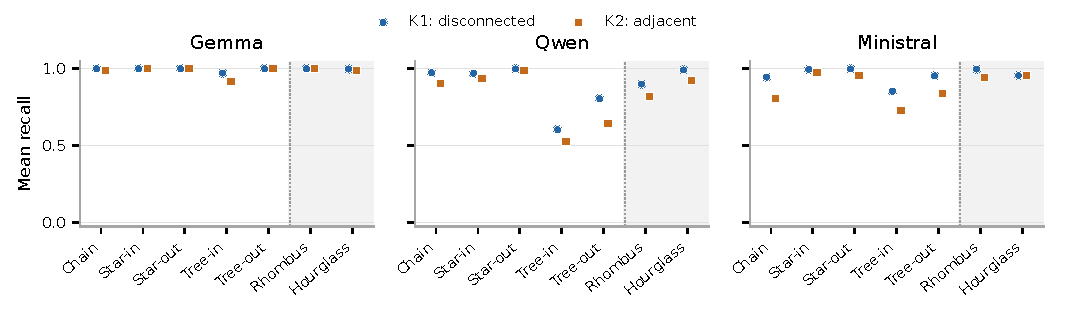
\includegraphics[width=\textwidth]{figures/recall_motifs.pdf}
\caption{Core recall with explicit source-card relations: K1 disconnected and K2 adjacent distractors, 100 planned tasks per point. The first five families have six nodes; shaded rhombus/hourglass use four/five and are not equal-size contrasts. Invalid outcomes contribute zero. These are descriptive macro means, without inferential error bars.}
\Description{Recall across seven graph-pattern families for three models. Incoming-tree recall is below outward-star recall, with model-dependent changes under adjacent contexts.}
\label{fig:motifs}
\end{figure*}

Figure~\ref{fig:motifs} shows task-family differences, including five families at the common six-node reference size. Under K1, six-node incoming-tree recall is 0.972 for Gemma, 0.603 for Qwen, and 0.853 for Ministral. Outward stars are close to complete coverage. The common size does not eliminate differences in query semantics, relation types, or sampled entities; it rules out a node-count-only description of these observed task profiles, not every competing explanation.

Precision supplies a different view. Qwen's K1 incoming-tree precision is 0.988, despite recall of 0.603 and exact recovery of 0.150. It often selects a small, mostly reference-consistent set while failing to cover the reference. Gemma's corresponding precision is 1.000 and exact 0.870. Appendix~\ref{app:conditions} reports precision profiles separately rather than combining the two quantities into one F1 curve.

\begin{figure*}[t]
\centering
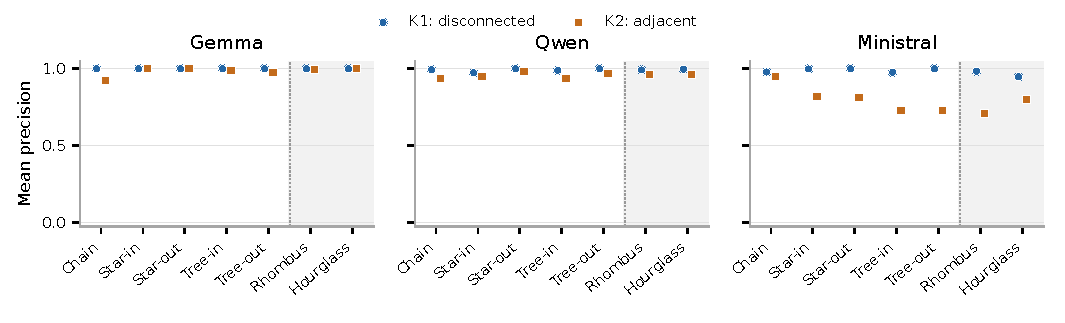
\includegraphics[width=\textwidth]{figures/precision_motifs.pdf}
\caption{Precision companion to Figure~\ref{fig:motifs}: Core K1/K2, 100 planned tasks per point, invalid zero. Shaded families have different sizes. High precision can coexist with incomplete coverage; this is a descriptive saved-score profile without confidence intervals.}
\Description{Precision across graph families, with near-ceiling disconnected scores for many cells and lower precision for several Ministral adjacent conditions.}
\label{fig:precisionmotifs}
\end{figure*}
\begin{figure*}[t]
\centering
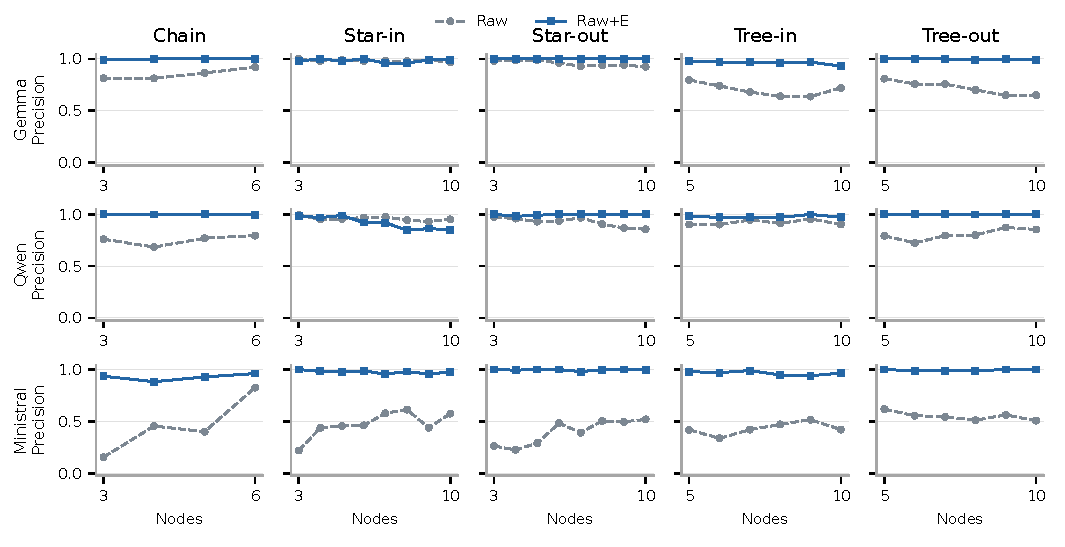
\includegraphics[width=\textwidth]{figures/precision_sizes.pdf}
\caption{Precision companion to Figure~\ref{fig:sizes}, retaining all three models and five variable-size families under Raw/Raw+E. Each point has 100 planned tasks; invalid contributes zero. Size cohorts differ and no curve is interpreted as a causal graph expansion.}
\Description{Precision over subgraph size. Explicit-overlay precision often remains high even where corresponding recall is incomplete.}
\label{fig:precisionsizes}
\end{figure*}

\begin{table}[t]
\caption{All Core condition means: recall, with 700 planned outcomes per model/condition and invalid zero. These are descriptive macro means.}
\label{tab:coreall}
\centering\small
\begin{tabular}{lrrr}
\toprule
Condition & Gemma & Qwen & Ministral \\
\midrule
K0 & 0.182 & 0.189 & 0.299 \\
K1 & 0.996 & 0.892 & 0.957 \\
K2 & 0.985 & 0.820 & 0.885 \\
K3 & 0.996 & 0.896 & 0.914 \\
K4 & 0.993 & 0.951 & 0.950 \\
K5 & 0.993 & 0.857 & 0.956 \\
K6 & 0.979 & 0.794 & 0.911 \\
K7 & 0.996 & 0.888 & 0.941 \\
K8 & 0.990 & 0.853 & 0.939 \\
K5k & 0.988 & 0.850 & 0.918 \\
R0 & 0.322 & 0.282 & 0.298 \\
R1-matched & 0.985 & 0.817 & 0.844 \\
R2-matched & 0.973 & 0.750 & 0.762 \\
\bottomrule
\end{tabular}

\end{table}
\begin{table}[t]
\caption{Precision counterpart to Table~\ref{tab:coreall}, using the same planned populations and failure policy.}
\label{tab:coreprecision}
\centering\small
\begin{tabular}{lrrr}
\toprule
Condition & Gemma & Qwen & Ministral \\
\midrule
K0 & 0.994 & 0.974 & 0.130 \\
K1 & 1.000 & 0.992 & 0.983 \\
K2 & 0.983 & 0.957 & 0.791 \\
K3 & 0.999 & 0.992 & 0.976 \\
K4 & 0.996 & 0.996 & 0.950 \\
K5 & 0.999 & 0.992 & 0.980 \\
K6 & 0.974 & 0.958 & 0.751 \\
K7 & 1.000 & 0.989 & 0.971 \\
K8 & 1.000 & 0.993 & 0.991 \\
K5k & 0.996 & 0.987 & 0.965 \\
R0 & 0.936 & 0.861 & 0.391 \\
R1-matched & 0.991 & 0.992 & 0.979 \\
R2-matched & 0.984 & 0.958 & 0.838 \\
\bottomrule
\end{tabular}

\end{table}

\paragraph{Output signatures and diagnostic limits.}
An exact one-hop signature means the saved selection equals the anchor plus all permitted first-hop neighbours. On the inspected Qwen K1 six-node incoming-tree tasks, this occurs in 71/100 outputs; K3/K4/K7 have 76/31/52. Their exact-reference counts are 16/51/16, compared with 15 in K1. This distinguishes elimination of a signature from correction of the task. All these Qwen cells have 100 valid outcomes. The same original 71 one-hop outputs become exact on 13 K3, 38 K4, and ten K7 tasks. Under K4, six initially exact outputs lose exactness. No new interval or significance test is attached to these post-hoc contrasts.

Ministral has 15/100 initial one-hop sets and 54/100 exact outputs in K1. K4 makes eight of those one-hop sets exact and loses exactness on nine initially exact tasks; total exact recovery is 62/100. Gemma's aggregate scores remain in all main tables/figures, but the archive lacks identities for this finer check. Output signatures do not prove hidden search depth or branch order.

On the inspected Qwen K1 incoming-tree inputs, undirected depth-two and directed depth-three coverage agree with the correct reference on all 100 tasks. Under K2 these alternative targets differ on 97/100 and 10/100 tasks, respectively; no Qwen output exactly matches those distinct alternative sets. This does not rule out mixed or partial rule violations. This slice has no terminal-type stopping condition, so it cannot diagnose terminal-type errors.

\paragraph{Analytical and uncertainty context.}
Select-all has recall one on every nonempty reference by definition, and precision equal to the reference proportion in the 25-candidate pool. These are analytical reference rules, not executed LLM/retrieval baselines. A full connected-component baseline was not computed. Earlier archive uncertainty analyses cover F1/exact with anchor-conditional assumptions; no such bands are reused for the present recall/precision results. Original exact scores, earlier metrics, native/legacy panels, and incomplete incremental histories remain in the supporting source artifacts rather than being pooled into the main populations.

\section{Author-Supplied Cypher Extraction Specification}
\label{app:cypher}
The following Cypher query was supplied by the authors for the appendix. Whitespace is normalized and comments are translated into English for display; executable tokens match the saved original. It enumerates small instances of nine directed pattern definitions, requires distinct vertices, and excludes additional directed typed edges inside each selected vertex set, including self-loops. The comparison uses source/type/target triples, so parallel physical relationships with the same triple are not distinguished by the extra-edge test.

This specification has fixed sizes: four-node chains/stars/rhombi, five-node trees/hourglasses, and three-node cycles/cliques. Its final \texttt{LIMIT 100} is global, not a quota per motif or size. It does not specify random sampling, seeds, candidate expansion, type/name acceptance filters, or the complete archived size grid. The presence of cycle/clique branches defines queries, not observed cycle/clique outcomes in the seven-family study. No result from executing these queries is claimed. These boundaries prevent equating the supplied query with a fully reconstructed historical pipeline. Cypher syntax is documented by Neo4j~\cite{neo4jCypher}.

\lstinputlisting{queries/author_query_english_comments.cypher}

The supplementary files include the existing queries for exporting nodes and edges and separately labelled, newly written frozen-instance checks. These supplementary files were not used to generate the reported outcomes. Graph-export code is not itself historical motif-extraction evidence. Query IDs and role bindings refer to the same database snapshot; \texttt{elementId} is not a portable cross-snapshot identifier.

\section{Directed Motifs and Query Rules}
\label{app:motifs}

We use seven directed task families, shown in the compact key in Figure~\ref{fig:raw_motifs}. Each query names an anchor $a$. An arrow $u\to v$ denotes a factual KG relation from $u$ to $v$; an incoming query examines this relation from $v$ toward $u$ without changing its direction. The endpoint answer set $A$ contains the entities returned by the query rule. The evaluated selection reference $W$ additionally includes the anchor and all intermediate entities on every permitted supporting route.

\paragraph{Chain.}
A directed path starts at the anchor. The query follows outgoing routes and stops at the first entity of the requested terminal type on each route. In the representative chain, the final vertex is that first matching entity; the vertices between the anchor and the final vertex are intermediate selections. The stopping rule is type-based, not a fixed two-link limit.

\paragraph{Star-in and star-out.}
The anchor is the common destination of the star-in edges and the common source of the star-out edges. The query requests all immediate incoming or outgoing neighbors, respectively. These neighbors are endpoint answers, while the anchor is additionally included in $W$.

\paragraph{Tree-in and tree-out.}
These families have two levels relative to the anchor, with at least two first-level branches and at least one second-level entity per branch. Tree-in edges point toward the anchor, while tree-out edges point away from it. The query inspects incoming or outgoing routes up to two links. A route ends earlier only when no further permitted unvisited neighbor is available. Second-level entities are endpoints in the representative Core examples; both levels and the anchor belong to $W$.

\paragraph{Rhombus.}
Four vertices form two outgoing two-link routes, $a\to b\to d$ and $a\to c\to d$. The endpoint answer is the shared vertex $d$, while $W=\{a,b,c,d\}$. Both intermediate vertices are required by the all-route selection convention even though the routes reach the same endpoint.

\paragraph{Hourglass.}
The central anchor has two incoming and two outgoing neighbors. The question requests these two one-link groups separately. The four neighbors are endpoint answers and all five vertices belong to $W$. The task does not ask for a two-link traversal from an incoming neighbor through the anchor to an outgoing neighbor.

The Core panel contains 100 base tasks per family: six nodes for chain, stars, and trees, four for rhombus, and five for hourglass; the size panel varies the supported chain, star, and tree sizes. Question templates use the anchor's name/type and the traversal/stopping rule. Procedural and direct formulations express the same endpoint query. Families therefore differ in query operations as well as directed structure, so their unadjusted profiles do not isolate a causal topology effect.


\end{document}
